\documentclass{article}[18pt]
\usepackage{../../../../format}
\lhead{A Level Maths - S2}

%File specific Preamble
\usetikzlibrary{positioning}

\begin{document}
\begin{center}
\underline{\huge Continuous Random Variables}
\end{center}
\begin{obeylines}
\section{Probability density function (PDF)}
The PDF describes how the probabilities are distributed over the range of values.
f(x) must satisfy these basic properties:
\begin{itemize}
\item $f(x)\geqslant 0$ for all values of $x$, so that no probabilities are negative.
\item $\mathlarger{\int_{\infty}^{-\infty}} f(x) dx=1$  (The sum of all probabilities is 1)
\item $P(a<x<b)=\mathlarger{\int_{a}^{b}} f(x) dx$
\end{itemize}
For continuous random variables $P(x<z)=P(x\leqslant z)$

\textbf{Example}
\end{obeylines}
$
  f(x)=\left\{
  \begin{array}{@{}ll@{}}
    \frac{1}{2}(x-3), & \text{for}\ 3\leq x \leq 5  \\
    0, & \text{otherwise}
  \end{array}\right.
$
\\
$\mathlarger{\int_{3}^{5}} \frac{1}{2}x-\frac{3}{2} \ dx = \Bigg[\dfrac{x^2}{4}-\dfrac{3x}{2}\Bigg]^5_3 = \Bigg(\dfrac{5^2}{4}-\dfrac{3\times5}{2}\Bigg)-\Bigg(\dfrac{3^2}{4}-\dfrac{3\times3}{2}\Bigg)=1$
\\
\textit{Find ${P(x<4)}$}\\
$\mathlarger{\int_{3}^{4}} \frac{1}{2}x-\frac{3}{2}\ dx = \Bigg[\dfrac{x^2}{4}-\dfrac{3x}{2}\Bigg]^4_3=0.25$\\
\textbf{Example 2}\\
$
  f(x)=\left\{
  \begin{array}{@{}ll@{}}
    x, & \text{for}\ 0\leqslant x \leqslant 1\\
    2-x, & \text{for}\ 1\leqslant x \leqslant 2\\
    0, & \text{otherwise}
  \end{array}\right.
$\\
$P(0.5<x<1.3)=\mathlarger{\int_{0.5}^{1} x \ dx+\int_{1}^{1.3} 2-x \ dx}= \Big[\frac{1}{2}x^2\Big]^1_{0.5}+\Big[2x-\frac{1}{2}x^2\Big]^1_{0.5}=0.63$
\section{Cumulative Distribution Function}
The CDF is $P(X\leqslant x)$\\
To find it, integrate the \textbf{PDF} between the lower limit and $x$.\\
\\
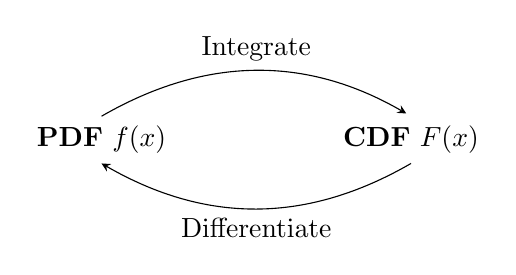
\begin{tikzpicture}
  \node (PDF) {\textbf{PDF} $f(x)$};
  \node[right=2cm of PDF] (CDF) {\textbf{CDF} $F(x)$};
  \draw[-stealth,shorten >= 2pt] (PDF.north) to[bend left] node[midway,above] {Integrate} (CDF.north);
  \draw[-stealth] (CDF.south) to[bend left] node[midway,below] {Differentiate} (PDF.south);
\end{tikzpicture}
\\
\\
\textbf{Example}\\
$
  f(x)=\left\{
  \begin{array}{@{}ll@{}}
    \frac{1}{2}(x-3), & \text{for}\ 3\leqslant x \leqslant 5\\
    0, & \text{otherwise}
  \end{array}\right.
$\\

$\mathlarger{\int_{3}^{x_0} \frac{1}{2}x-\frac{3}{2} \ dx= \Bigg[\dfrac{x^2}{4}-\dfrac{3x}{2}\Bigg]^1_{0.5}}=
\Bigg(\dfrac{x^2}{4}-\dfrac{3x}{2}\Bigg)-\Bigg(\dfrac{3^2}{4}-\dfrac{3\times 3}{2}\Bigg)=\dfrac{x^2}{4}-\dfrac{3x}{2}+\dfrac{9}{4}$\\
$
  F(x)=\left\{
  \begin{array}{@{}ll@{}}
  	0, & \text{for}\ x<3\\
    \frac{x^2}{4}-\frac{3x}{2}+\frac{9}{4}, & \text{for}\ 3\leqslant x \leqslant 5\\
    1, & \text{for}\ x>5
  \end{array}\right.
$\\
\newpage
\textbf{Example 2}\\
$
  f(x)=\left\{
  \begin{array}{@{}ll@{}}
    x, & \text{for}\ 0\leqslant x \leqslant 1\\
    2-x, & \text{for}\ 1\leqslant x \leqslant 2\\
    0, & \text{otherwise}
  \end{array}\right.
$\\
\textit{Find the CDF}\\
\\
$\mathlarger{\int_{0}^{x}} x\ dx = \Bigg[\dfrac{x^2}{2}\Bigg]^x_0=\dfrac{x^2}{2}$\\
$F(1)+\mathlarger{\int_{1}^{x}} 2-x\ dx =\dfrac{1^2}{2}+ \Bigg[2x-\dfrac{x^2}{2}\Bigg]^x_1=\dfrac{1}{2}+\Big((2x-\dfrac{x^2}{2})-(2-\dfrac{1}{2})\Big)=2x-\dfrac{x^2}{2}-1$\\
$
  f(x)=\left\{
  \begin{array}{@{}ll@{}}
    0, & \text{for}\ x<0\\
    \frac{x^2}{2}, & \text{for}\ 0\leqslant x \leqslant 1\\
    2x-\frac{x^2}{2}-1, & \text{for}\ 1\leqslant x \leqslant 2\\
    1, & \text{for}\ x>2
  \end{array}\right.
$\\
\section{Mean and variance of continuous random variables}
Mean$=\mu=E(x)=\mathlarger{\int_{a}^{b}}xf(x)\ dx$ for $a\leqslant x\leqslant b$\\
$\text{Var}(x)=E(x^2)-(E(x))^2$\\
$E(x^2)=\mathlarger{\int_{a}^{b}}x^2f(x)\ dx$









\end{document}